%________________________________________________________________________________________
% @brief    LaTeX2e Resume for Kamil K Wojcicki
% @author   Kamil K Wojcicki
% @url   http://linux.dsplabs.com.au/?p=54
% @date     Decemebr 2007
% @info     Based on Latex Resume Template by Chris Paciorek 
%        http://www.biostat.harvard.edu/~paciorek/
%________________________________________________________________________________________
\documentclass[margin,line,a4paper]{resume}

\usepackage[utf8]{inputenc} %utf8
\usepackage[english,danish]{babel}
\usepackage[T1]{fontenc}
\usepackage{graphicx,wrapfig}
\usepackage{url}
\usepackage[colorlinks=true, a4paper=true, pdfstartview=FitV,
linkcolor=blue, citecolor=blue, urlcolor=blue]{hyperref}
% \pdfcompresslevel=9
\usepackage{wx672cjk}


\begin{document}
{\sc \Large 蒲启元}
\begin{resume}
    \vspace{0.5cm}
    \begin{wrapfigure}{R}{0.6\textwidth}
        \vspace{-1cm}
       \begin{center}
       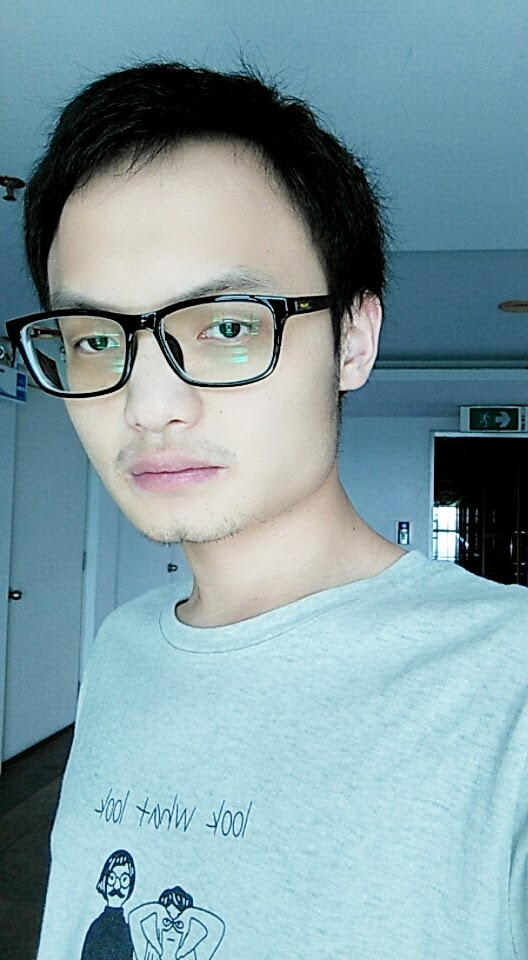
\includegraphics[width=0.3\textwidth]{me1}
       \end{center}
        \vspace{-1cm}
    \end{wrapfigure}
    


    \section{\mysidestyle 个人\\信息}%\vspace{2mm}
    蒲启元 \\
    手机: 18314555392 \\
    Email: pqy7172@gmail.com \\
    \href{https://github.com/Puqiyuan}{Github}\\    

    蒲启元,1995年12月生,四川南充人。计算机科学与技术专业毕业,2014---2015年度校级三好学
    生,2015---2016年度省级三好学生,优秀毕业生,优秀毕业设计,2018年云南省大学生计算机作
    品赛二等奖。泰国交换生,四六级证书,英语阅读、口语、写作良好。

    RongOS简单操作系统开发者,具有良好的编程基础,ACM-ICPC爱好者,满分通过很多清华判题系统、
    URI判题系统中的题目。Programming SWFU编程兴趣小组发起人,热衷于帮助西南林业大学同学体
    验到编程的快乐。主要专业课比如数据结构,操作系统等全部90分以上。具有较强的自学能力,善
    于使用Google解决各种问题。
    


\end{resume}
\end{document} 



%%% Local Variables:
%%% mode: latex
%%% TeX-master: t
%%% End:
